\documentclass[12pt]{amsart}
\usepackage{geometry}                % See geometry.pdf to learn the layout options. There are lots.
\geometry{letterpaper}                   % ... or a4paper or a5paper or ... 
\usepackage{float}
\usepackage{url} 


\usepackage{tikz}			    % This package allows us to do a LOT of graphics stuff. Google Tikz


\setlength{\evensidemargin}{.75in}
\addtolength{\evensidemargin}{-1in}
\setlength{\oddsidemargin}{.5in}
\addtolength{\oddsidemargin}{-1in}
\setlength{\topmargin}{.75in}
\addtolength{\topmargin}{-1.25in}
\setlength{\textwidth}{7.5in}
\setlength{\textheight}{10in}
\linespread{1}


\pagestyle{empty}
\setlength{\oddsidemargin}{0.3in} 
\setlength{\textheight}{8in}
\setlength{\topmargin}{0.4in}
\setlength{\headsep}{0in}
\setlength{\parskip}{0pt}
\setlength{\parindent}{0pt}
\setlength{\textwidth}{5.9in}
\font\Bbb=msbm10                 %outline bold character 
\newcommand{\RR}{\hbox{\Bbb R}}
\newcommand{\CC}{\hbox{\Bbb C}}
\newcommand{\QQ}{\hbox{\Bbb Q}}
\newcommand{\NN}{\hbox{\Bbb N}}
\newcommand{\ZZ}{\hbox{\Bbb Z}}
\newcommand{\kk}{\hbox{\bf k}}
\newcounter{probnum}
\partopsep 0pt
\settowidth{\leftmargini}{1.}\addtolength{\leftmargini}{\labelsep}
\newenvironment{prob}{\begin{enumerate}\setcounter{enumi}{\value{probnum}}}%
 {\setcounter{probnum}{\value{enumi}}\end{enumerate}}
\settowidth{\leftmarginii}{(a)}\addtolength{\leftmarginii}{\labelsep}
\newenvironment{subprob}{\begin{enumerate}\topsep 0pt}{\end{enumerate}}
\renewcommand{\theenumiii}{\roman{enumiii}}
\renewcommand{\labelenumiii}{(\theenumiii)}
\settowidth{\leftmarginiii}{(viii)}\addtolength{\leftmarginiii}{\labelsep}
\newenvironment{ssubprob}{\begin{enumerate}}{\end{enumerate}}
\def\heading#1{\vskip\bigskipamount\hfill{\sc #1}\hfill}

\begin{document}

\begin{center}
{\large \sc 
ASSIGNMENT 2 - MATH 4090 (Winter 2022)} \\
\  \\
{\sc  STUDENT:} Francis Calingo (214451736)\\

 \end{center}
\vspace{.5in}

\noindent {\bf Question 1}:  

\begin{prob}

  \item[a.] {\bf Modelling Careers}
  
  \noindent Some examples of careers that require mathematical modelling include machine learning scientists (a position Dr. Michael Akinwumi occupies),  AI engineer (a position John Murdoch occupies), health economist (something Dr Angie Read specializes in), risk analyst, and methodologist.

  \noindent According to a US News report, mathematicians can make 80,000 to 120,000 per year in 2020. 
  
  \url{https://money.usnews.com/careers/best-jobs/mathematician/salary}
  
  \item[b.] {\bf Arms Race}

  \noindent Given that an increased distrust correlates to more militarization, a positive parameter means higher distrust, a negative parameter means lower distrust, and 0 means neutral.
  
\noindent In most cases, there will be a runaway arms race. However, for certain parameters, there will be a stabilized arms race. Take, for example, a=-7.5 and b=9. Country x's military spending stabilizes slightly around 4.25 and Country y's spending stabilizes around 1.75. If we were to slightly increase a or b, it immediately becomes a runaway race or shows an impossible scenario (i.e., spending approaches negative infinity).

\bigskip 
\begin{center}
    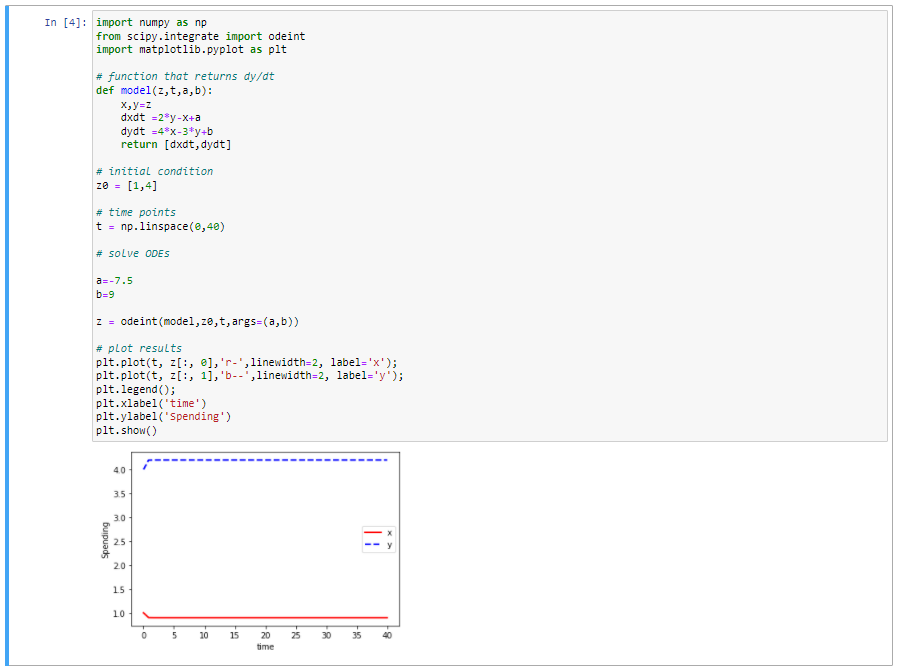
\includegraphics[width=6cm]{Q1_1A.png}
    \vspace{0.5em}
    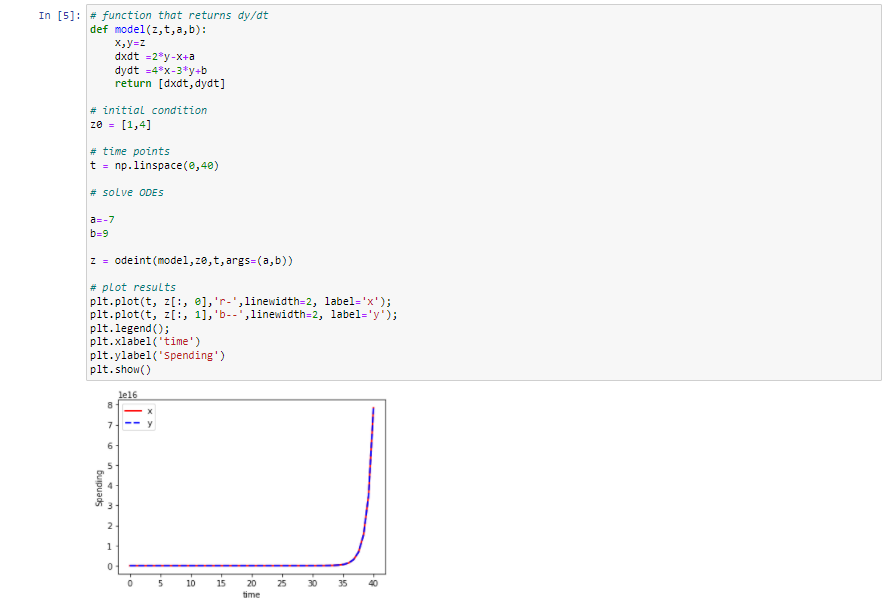
\includegraphics[width=6cm]{Q1_1B.png}
    \vspace{0.5em}
    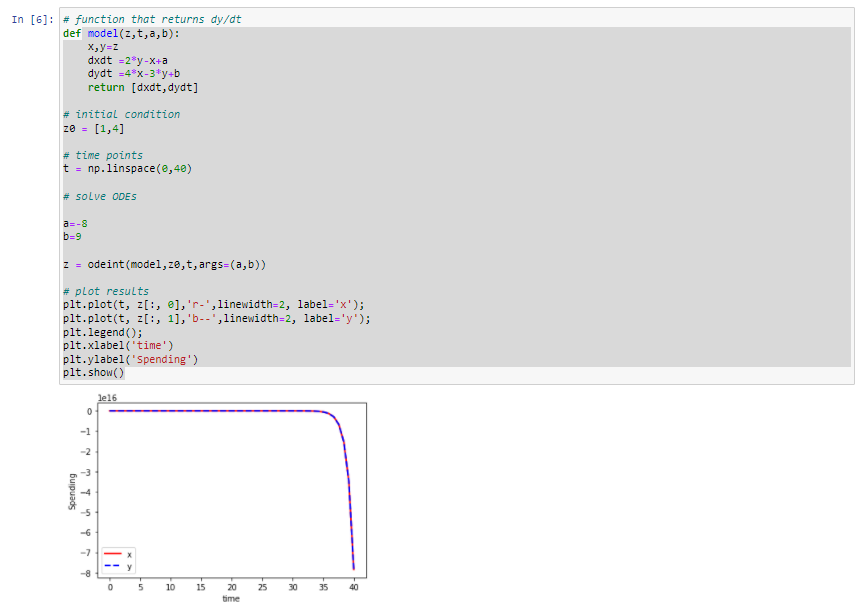
\includegraphics[width=6cm]{Q1_1C.png}
    \vspace{0.5em}
    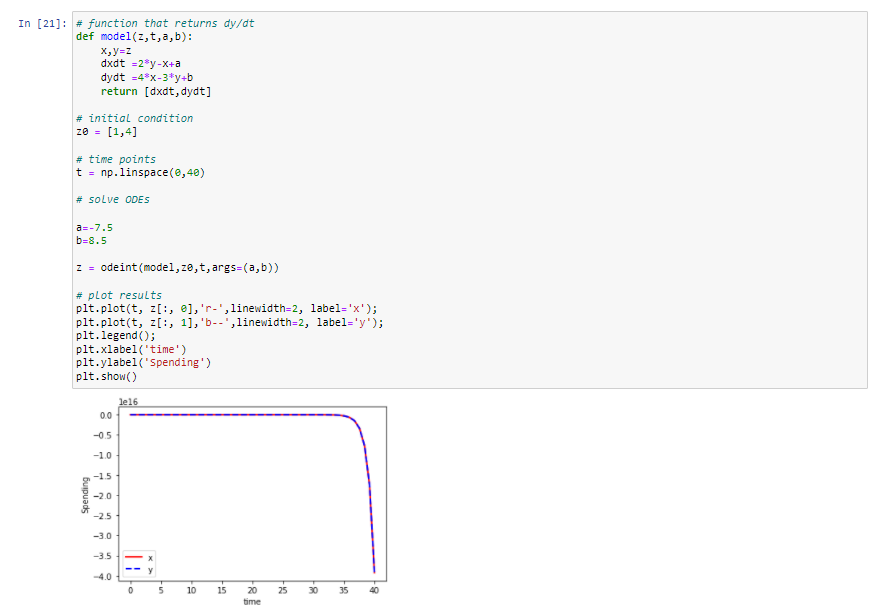
\includegraphics[width=6cm]{Q1_1D.png}
    \vspace{0.5em}
    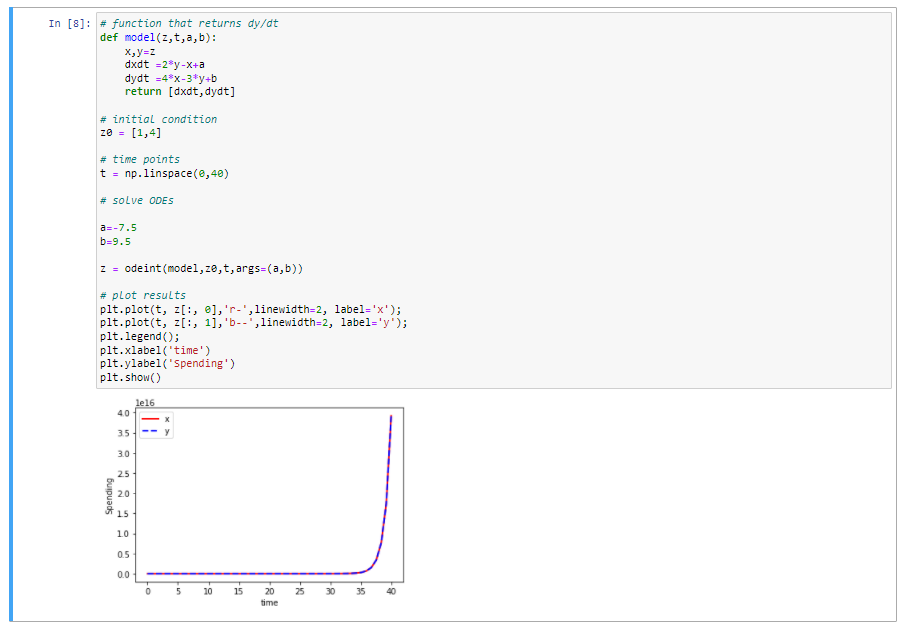
\includegraphics[width=6cm]{Q1_1E.png}
\end{center}

\noindent When a=b=-2, both countries' spending stabilizes around 2. Now observe that if we decrease a by 0.5 and increase b by 1, the arms race will still be stabilized, but Country Y's spending begins to outpace Country x's until x and y have constant spending (4 and 1, respectively) when a=-7 and b=9. This makes sense because since Country x has a low distrust of Country y, it's spending is much less. Conversely, Country y's strong distrust of x means its spending will vastly outpace x's.

\bigskip 

\begin{center}
    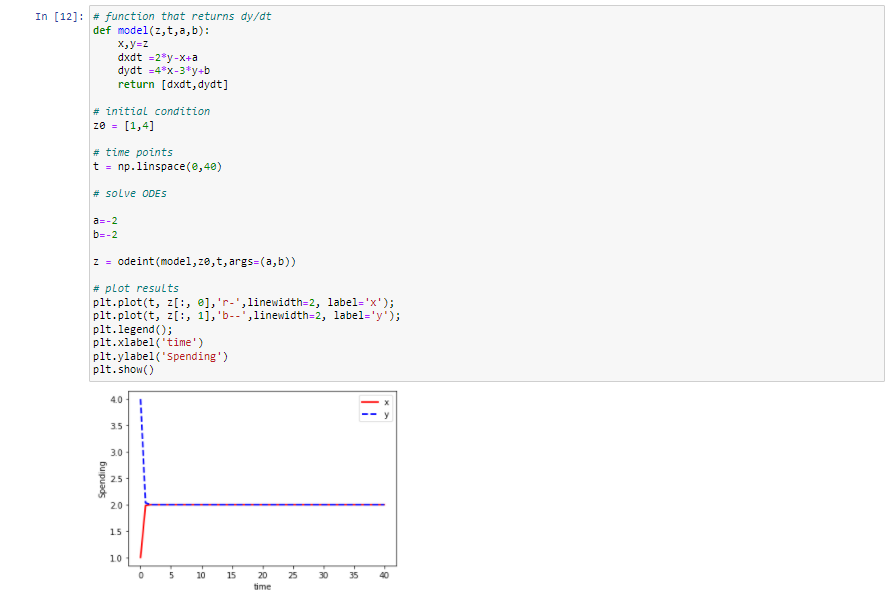
\includegraphics[width=6cm]{Q1_1F.png}
    \vspace{0.5em}    
    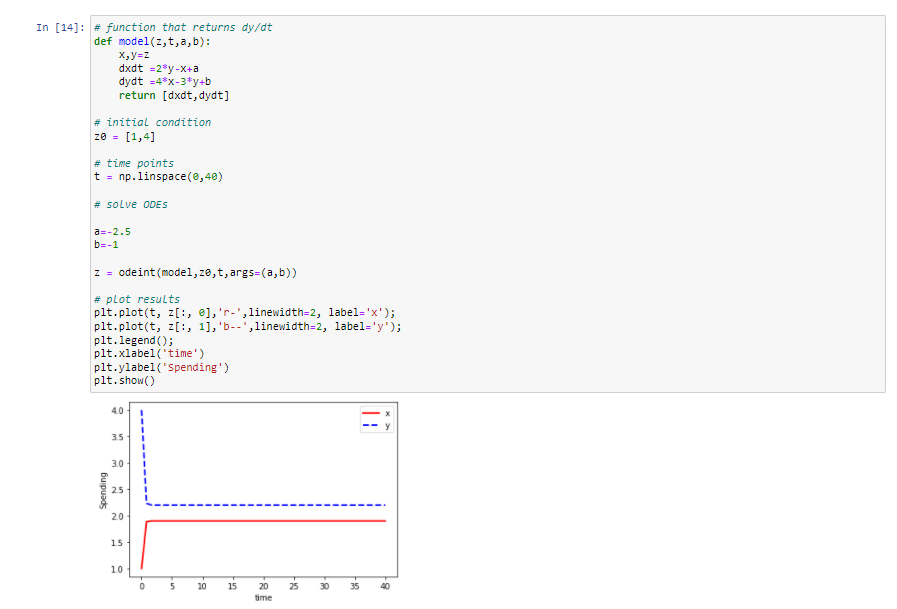
\includegraphics[width=6cm]{Q1_1G.png}
    \vspace{0.5em}    
    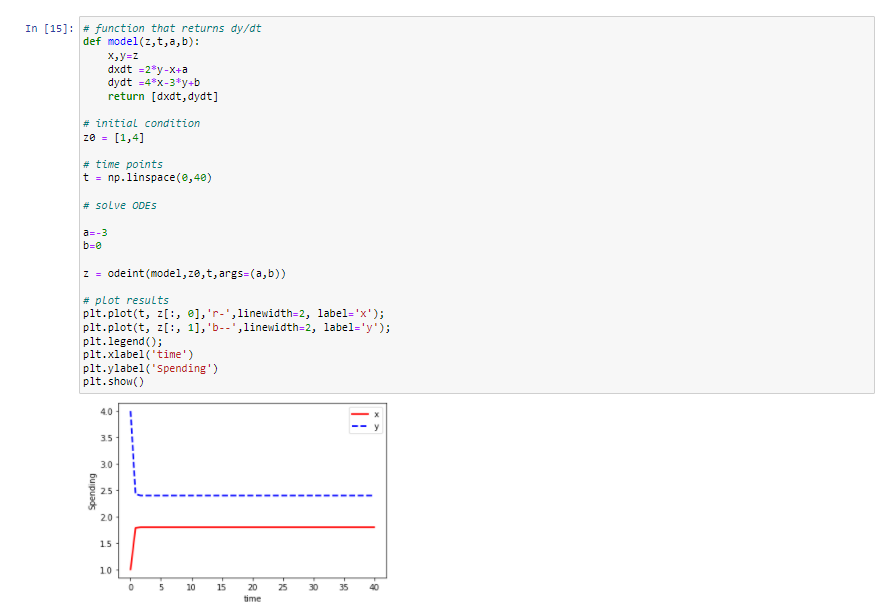
\includegraphics[width=6cm]{Q1_1H.png}
    \vspace{0.5em}    
    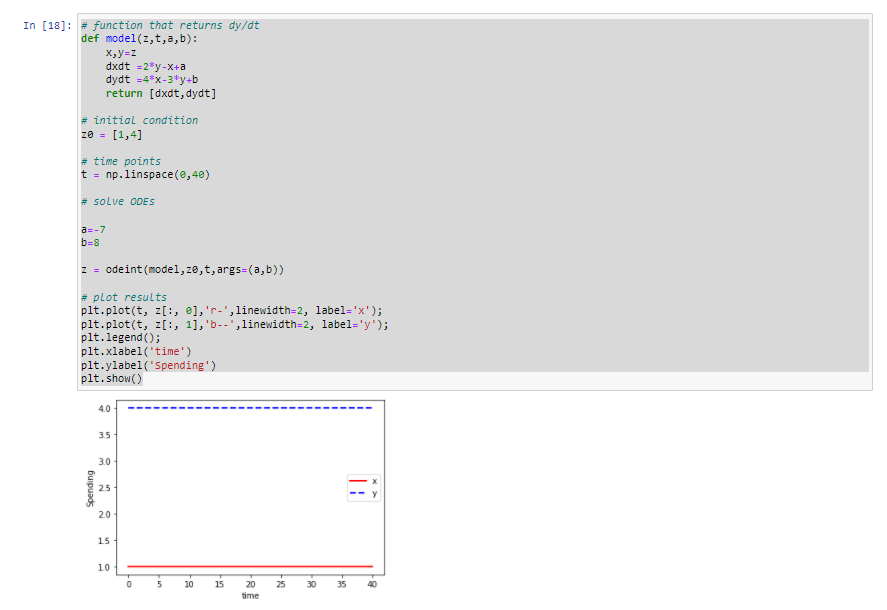
\includegraphics[width=6cm]{Q1_1I.png}
\end{center}

\noindent Let's start again at a=b=-2. Now observe that if we increase a by 0.5 and decrease b by 1, the arms race will still be stabilized, but Country x's spending begins to outpace Country y's. Again, this makes sense because as Country x's distrust increases, so does its spending, while as Country y's distrust decreases, so does its spending. Of course, we cannot keep decreasing/increasing that way, as the model will eventually reach negative spending, which is of course impossible.

\begin{center}
    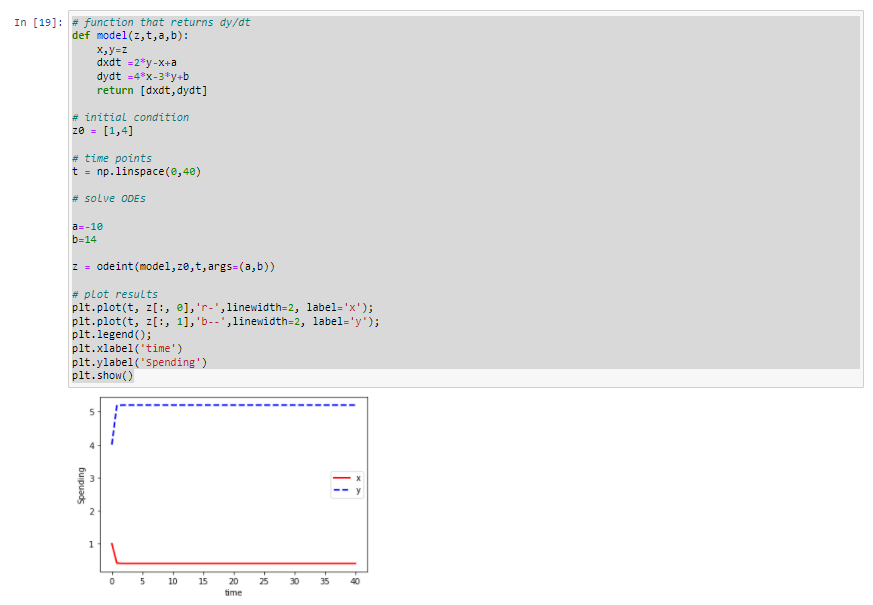
\includegraphics[width=6cm]{Q1_1J.png}
    \vspace{0.5em} 
    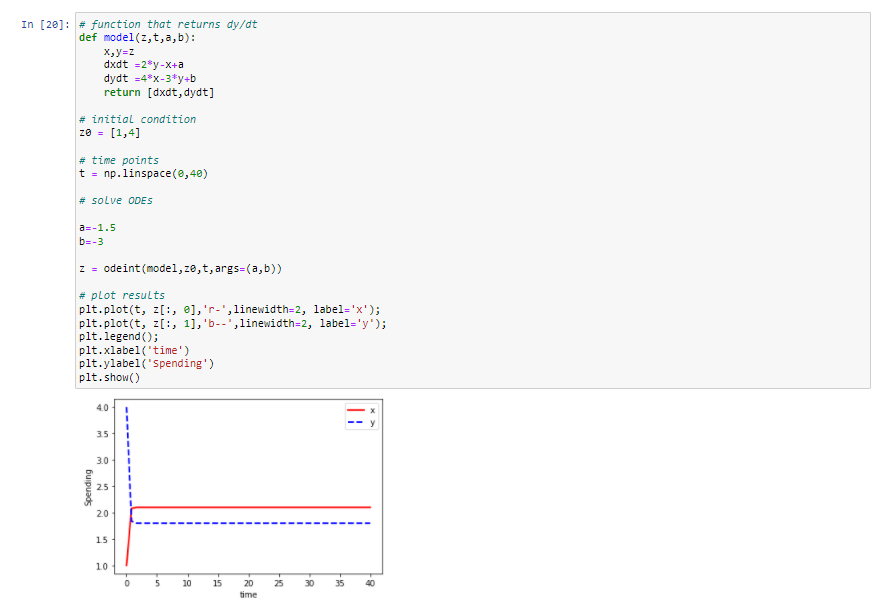
\includegraphics[width=6cm]{Q1_1K.png}
    \vspace{0.5em} 
    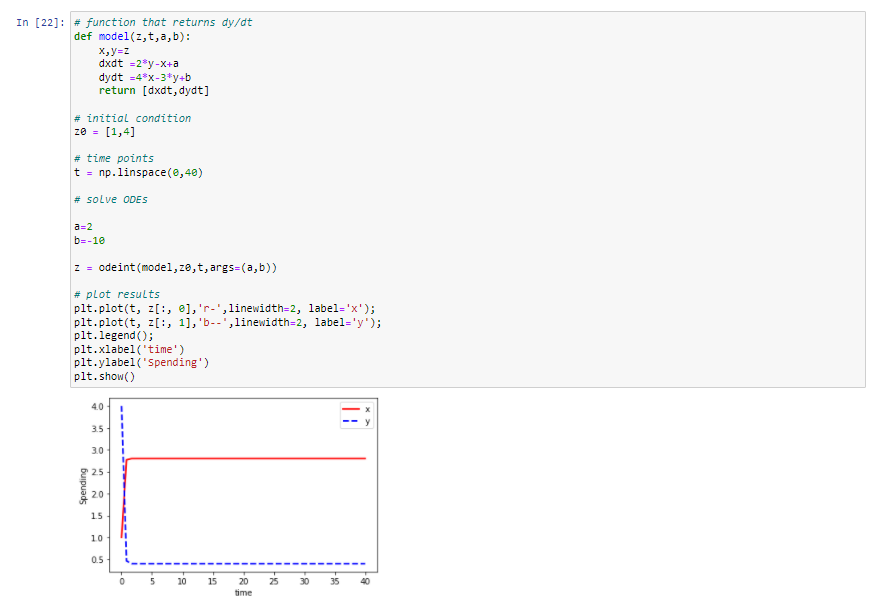
\includegraphics[width=6cm]{Q1_1L.png}
    \vspace{0.5em} 
    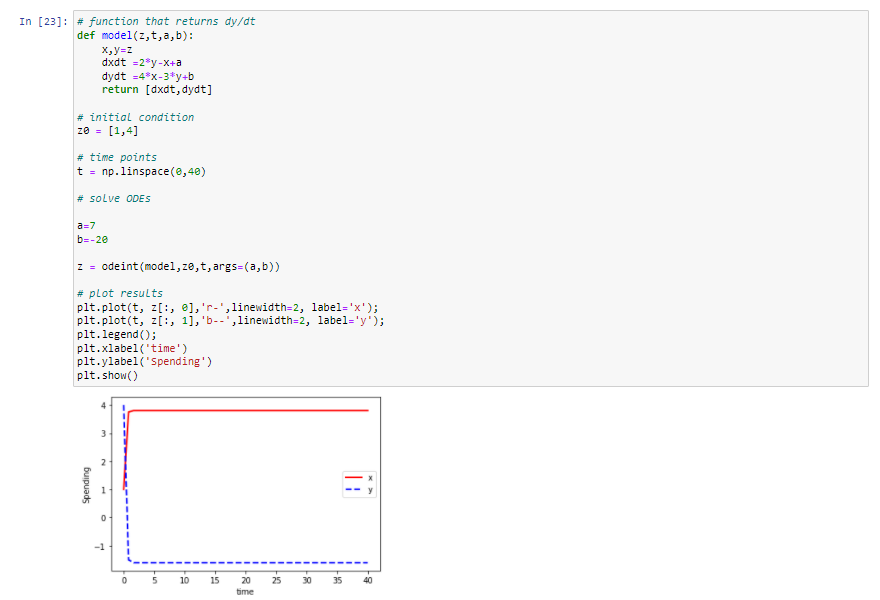
\includegraphics[width=6cm]{Q1_1M.png}
    
\end{center}
  
  \item[c.] {\bf Combat }
  
  \noindent According to the results, conventional troops will win since over time, x1 will approach some constant slightly less than 6, but x2 will approach 0. This mode therefore supports the belief that because conventional troops are generally better trained, more well-equipped, and have better tactics, they will beat the guerrillas over time.
  
  \bigskip 
\begin{center}
    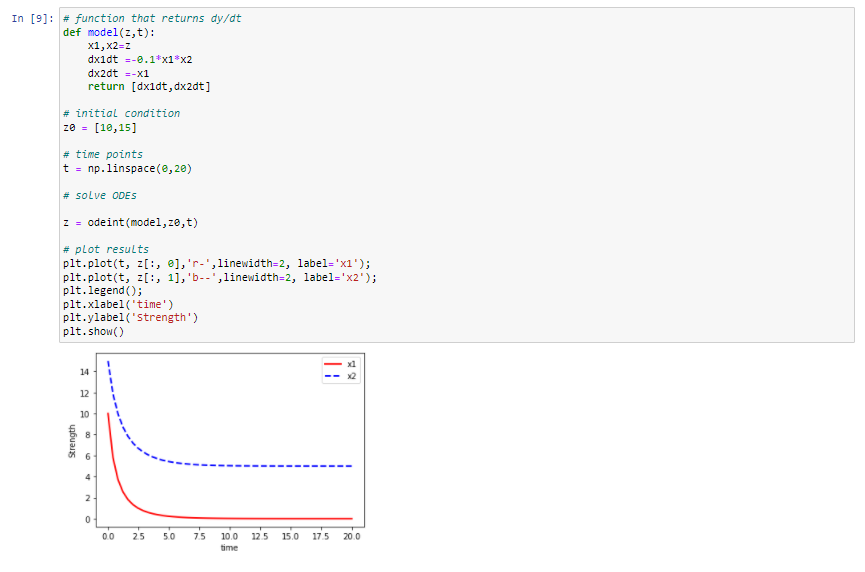
\includegraphics[width=6cm]{Q1_2.png}
\end{center}
  
 \end{prob}

\noindent {\bf Question 2}:  

\begin{prob}
\item[a.] {\bf Predator Prey}
  
  \noindent For x0=2 and y0=4, the first graph is x and y plotted against t, and the second is x plotted against y.

\begin{center} 
    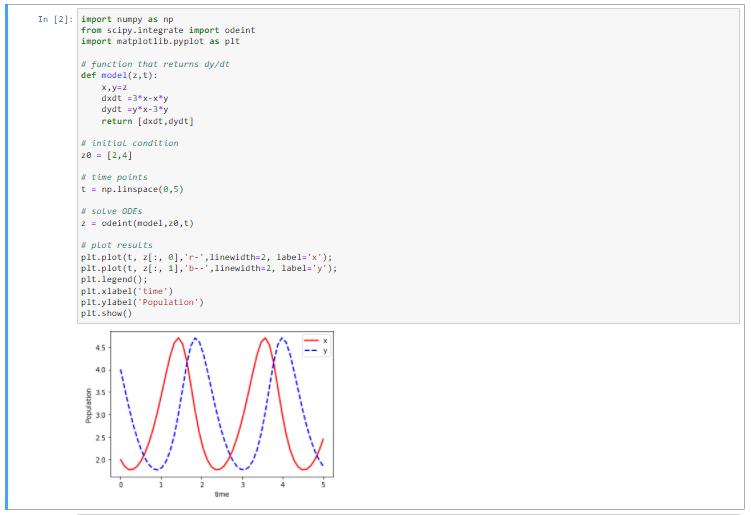
\includegraphics[width=6cm]{Q2_1.png}
    \vspace{0.5em} 
    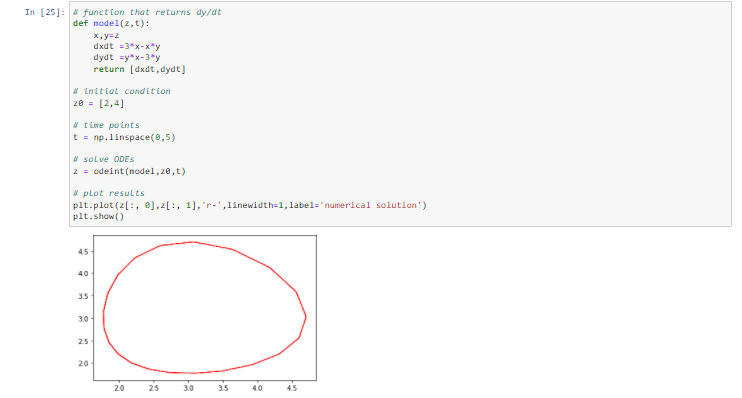
\includegraphics[width=6cm]{Q2_2.png}

\end{center}
    
\noindent As expected, the first graph is periodic, given that prey population declines as predator population increases, but that trend reverses, when there is little prey for the predators to eat. The second graph is an ellipse, as expected when graphing x against y.
    
\noindent For x0=2 and y0=5, the first graph is x and y plotted against t, and the second is x plotted against y.
  
\begin{center} 
    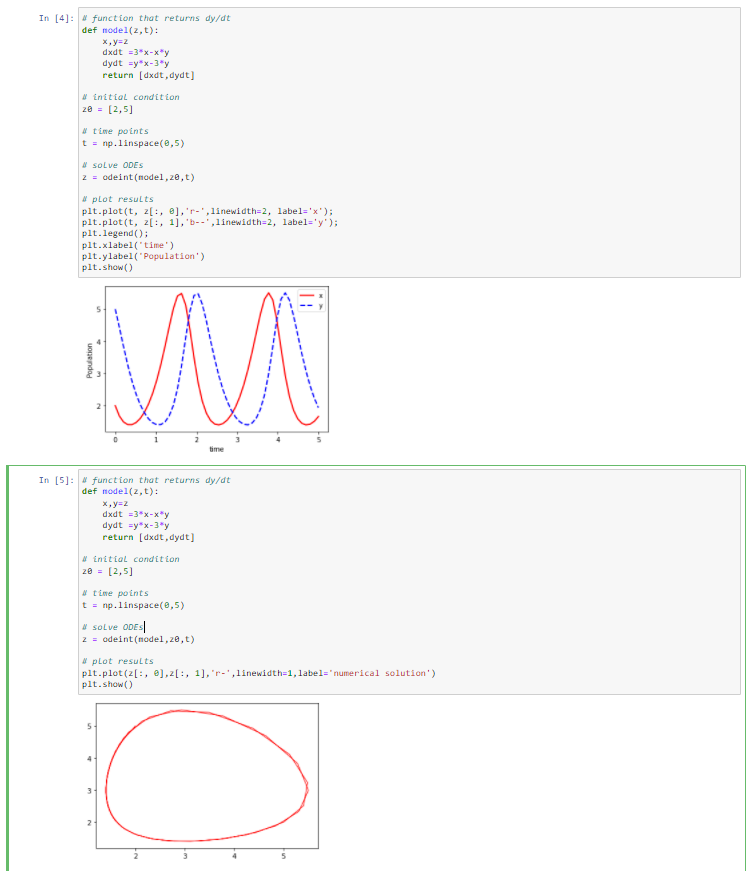
\includegraphics[width=6cm]{Q2_3.png}
\end{center}
\noindent  For x0=2 and y0=7, the first graph is x and y plotted against t, and the second is x plotted against y.
  
\begin{center} 
    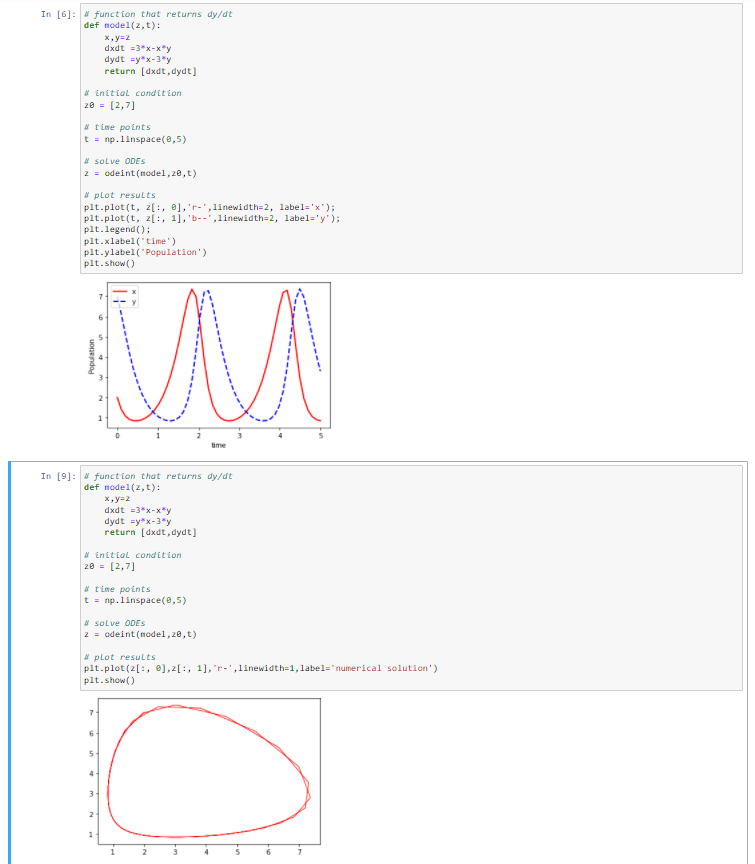
\includegraphics[width=6cm]{Q2_4.png}
\end{center}
\noindent Observe that as y0 increases, there is a significant change in the dynamics of x and y. x's declines and y's growth are much steeper, with the reverse being true for their growth and declines, respectively. As a result, the x vs y plot is less smooth.

\bigskip 
 \item[b.] {\bf Competing Species}
  
\begin{center} 
    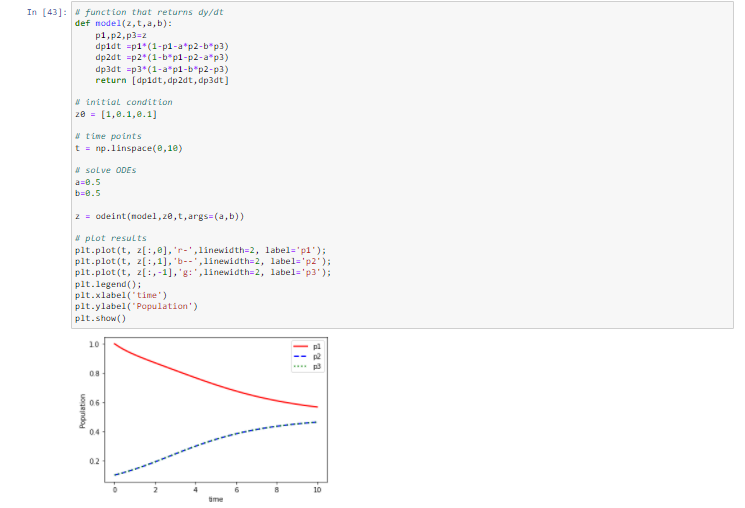
\includegraphics[width=6cm]{Q2_5.png}
    \vspace{0.5em} 

    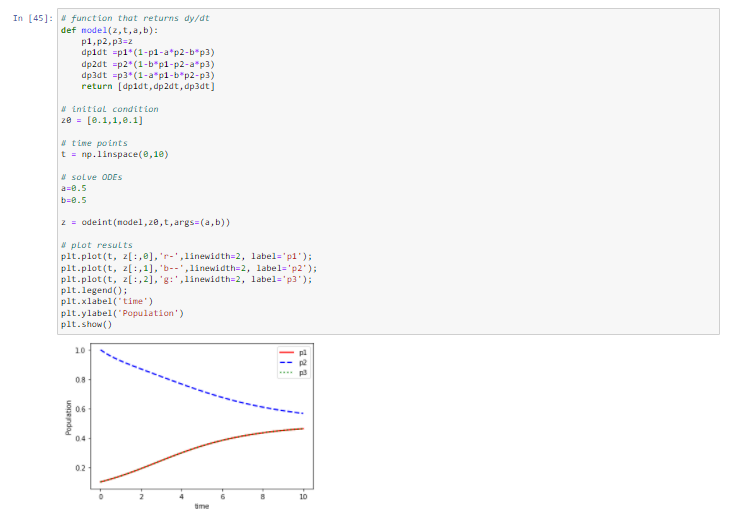
\includegraphics[width=6cm]{Q2_6.png}
    \vspace{0.5em} 

    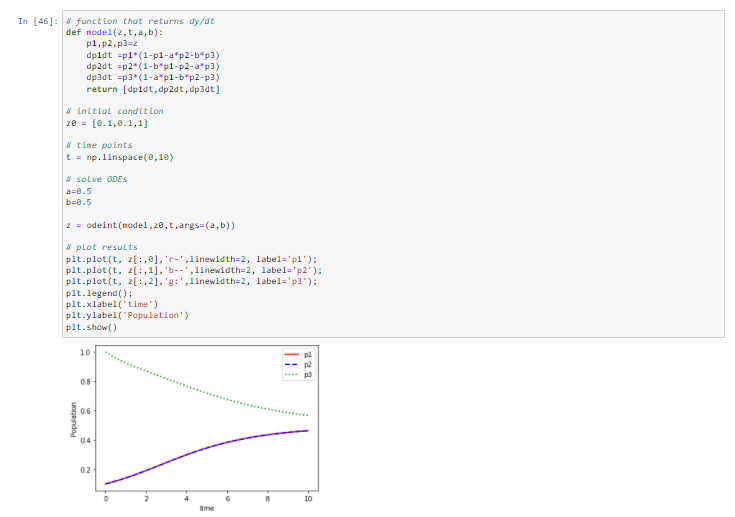
\includegraphics[width=6cm]{Q2_7.png}
\end{center}
  
  \noindent In each situation, two of the three Si's will have the same increasing behaviour, while the 3rd one is decreasing. In all cases, as t approaches infinity, all species will approach equilibrium. It appears that that they will approach a stable population of 0.5.


 \end{prob}

 \noindent {\bf Question 3}:  

\begin{prob}
  
  \bigskip 
  
  \item[a.] {\bf SIR Model}
  
  \noindent We can visualize the model as something like:
  
  \noindent $S \rightarrow I \rightarrow R$
  
  \noindent Since recoveries is dependent on the survival of infected individuals, then [change in R] $\alpha$ [change in I] so  we have
  
  \noindent $\frac{\delta R}{\delta t}$=qI, where q is a parameter.
  
  \noindent Now recall that in the predator-prey model, where x is prey and y is predator, $\frac{\delta x}{\delta t}$=$ax-dxy$, where a is the growth rate of x and d is the death rate of x.
  
  \noindent We can treat I as predator and S as prey. Of course, there will be no growth for S since it will either decrease or remain the same as people get infected. Also, there is N population. Therefore, we can say that $\frac{\delta S}{\delta t}$=$-\frac{pSI}{N}$, where p is a parameter.
  
  \noindent Using the predator-prey model again, we have that $\frac{\delta y}{\delta t}$=$\beta xy-ky$, where $\beta$ is the growth rate for predator and k is the death rate. Treating  I as "predator" and S as "prey", we have that $\frac{\delta I}{\delta t}$=$\frac{pSI}{N}$-$qI$. Think of q as the rate in which the infected decrease (i.e., recover), and p as the rate in which the infected increase (i.e., S becomes infected).
  
  \bigskip
  
  \noindent $\frac{\delta S}{\delta t}$=$-\frac{pSI}{N}$
  
  \noindent $\frac{\delta I}{\delta t}$=$\frac{pSI}{N}$-$qI$
  
  \noindent $\frac{\delta R}{\delta t}$=qI
  
  \noindent N=763
  
  \noindent S(0)=N-1=762
  
  \noindent I(0)=1 (patient zero required to start an outbreak).
  
  \noindent R(0)=0 (no one has recovered yet because 762 people have not been infected and there is 1 active case).

\bigskip 

 \item[b.] {\bf Parameters Estimates}
  \bigskip 
  
  \noindent Since N is a known parameter in this case, we'll have to estimate p and q. After testing several values, I chose p= and q= since the model looked like it made sense visually (the peak of I is around Day 7 and is around Infected Student=285). Also, I is near 0 at Day 15. The shape of I matches what an active cases model should look like, increasing until it reaches a certain point, then decreasing as recoveries outnumber infections and as epidemiological controls slows down the decrease of susceptible population.

\begin{center} 
    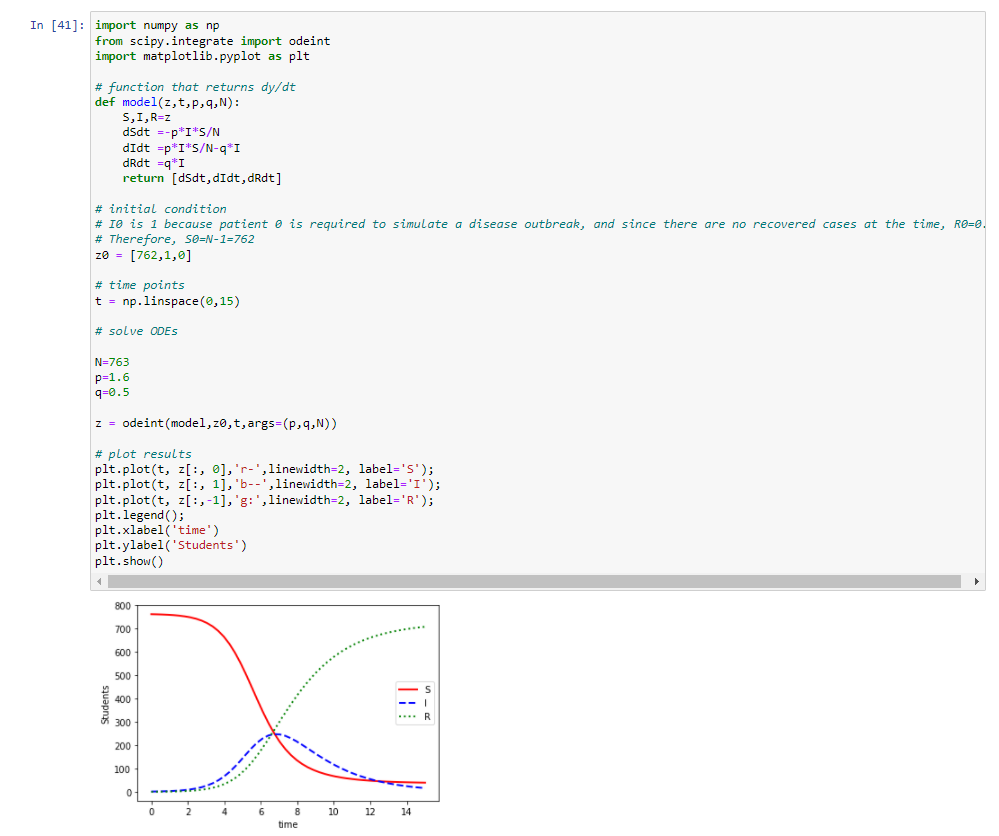
\includegraphics[width=6cm]{Q3_1.png}
\end{center}
    
     \item[c.] {\bf Goodness of Fit}
  
  \noindent $R^2$ is a goodness of fit measure that can be used because it's a metric that measures how well the data fits the model. Mathematically it's denoted by $1-\frac{SS Residuals}{SS Total}$.
  
\begin{center} 
    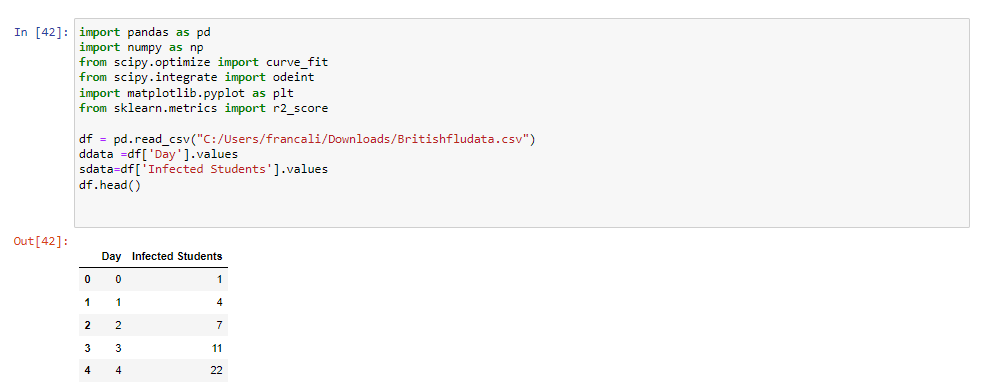
\includegraphics[width=6cm]{Q3_2A.png}
    \vspace{0.5em} 
    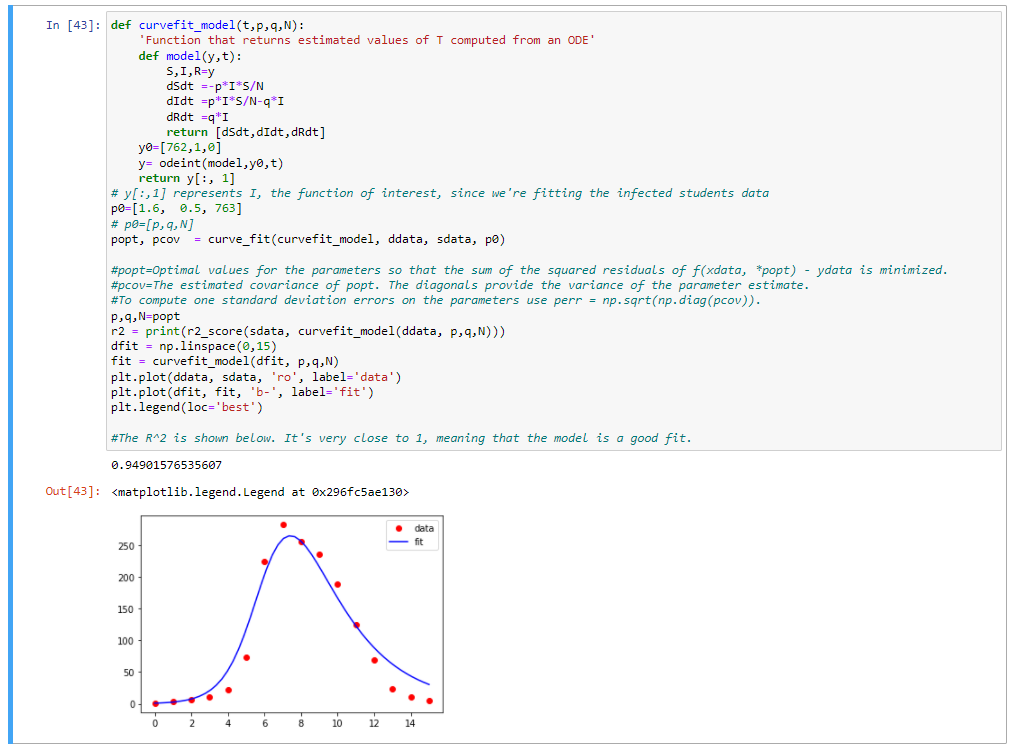
\includegraphics[width=6cm]{Q3_2B.png}
    \end{center}
    
\item[d.] {\bf Sensitivity}

\begin{center} 
    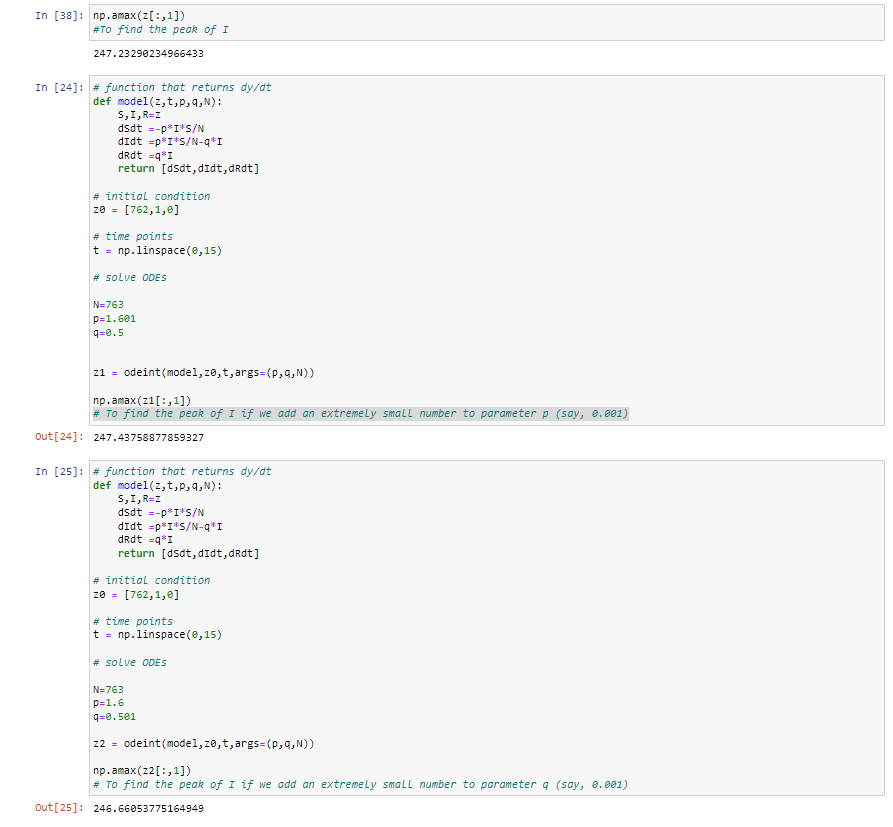
\includegraphics[width=6cm]{Q3_3A.png}
\end{center}
    
    \noindent Sensitivity of peak with respect to p is 
    
    $\frac{Peak(p+\Delta p)-Peak(p)}{\Delta p}$*$\frac{p}{Peak(p)}$=$\frac{Peak(1.6+0.001)-Peak(1.6)}{0.001}$*$\frac{1.6}{Peak(1.6)}$=$\frac{247.438-247.233}{0.001}$*$\frac{1.6}{247.233}$
    
    =1.327
    
    \bigskip
    
    \noindent Sensitivity of peak with respect to q is 
    
    $\frac{Peak(q+\Delta q)-Peak(q)}{\Delta q}$*$\frac{q}{Peak(q)}$=$\frac{Peak(0.5+0.001)-Peak(0.5)}{0.001}$*$\frac{0.5}{Peak(0.5)}$=$\frac{246.661-247.233}{0.001}$*$\frac{0.5}{247.233}$
    
    =-1.157
    
    \bigskip
    
    \noindent Both p and q have the same but opposite effect. This was confirmed when I was testing different parameters. Increasing one of the parameters moved the peak down, but increasing the other moved the peak right.


 \end{prob}
 
 \end{document}
